% =============================================================================
% CHAPITRE 2 - Revue de la littérature
% Refonte 2026-05-05 selon documentation/memoire/plan_refonte_revue_litterature.md
% Structure cible : 7 sections (2.1 à 2.7), 25-35 pages, fil rouge inversé.
% Source d'archive : consigne/revue_litterature_v2_DSR.tex (à ne pas toucher).
% =============================================================================

\chapter{Revue de la litt\'erature}\label{chap:revue}

Dans une démarche de Design Science Research, la revue de littérature ne sert pas seulement à recenser des travaux existants. Elle doit aussi construire le problème de recherche, identifier les connaissances disponibles pour y répondre, puis faire apparaître le manque que l'artefact devra combler (Hevner et al., 2004 ; Peffers et al., 2007 ; Gregor et Hevner, 2013). Le fil directeur retenu dans ce chapitre est donc le suivant : les organisations ne cherchent pas uniquement à savoir si des modèles de langage peuvent produire du code ou exécuter des tâches ; elles cherchent à savoir comment organiser, gouverner et évaluer des collectifs hybrides composés d'humains, d'agents LLM et d'artefacts numériques partagés.

Ce déplacement est central. Les premiers usages de l'IA générative ont surtout été analysés sous l'angle de la productivité individuelle, par exemple l'accélération de certaines tâches de développement logiciel ou l'aide à l'exploration de problèmes mal définis (Peng et al., 2023 ; Barke et al., 2023). Mais lorsque ces usages deviennent organisationnels, le problème change de nature. Il ne s'agit plus seulement de produire plus vite ; il s'agit de maintenir une capacité collective à décider, contrôler, corriger, tracer et apprendre. La question devient donc managériale autant que technique : comment bénéficier de l'autonomie agentique sans perdre la maîtrise du système d'information, de ses coûts, de sa conformité et de ses responsabilités ?

Le chapitre progresse en sept temps. La section 2.1 part du défi managérial posé par l'industrialisation de l'IA générative agentique et montre pourquoi les architectures logicielles héritées en constituent un révélateur particulièrement exigeant. La section 2.2 définit les conditions de gouvernabilité d'une écologie agentique : supervision humaine, auditabilité, guardrails, conformité, responsabilité et sécurité. La section 2.3 mobilise les théories de la coordination organisationnelle, des capacités dynamiques, des routines et des affordances pour établir le vocabulaire managérial du problème. La section 2.4 introduit alors la stigmergie, non comme une métaphore biologique isolée, mais comme un mécanisme de coordination indirecte susceptible de répondre aux exigences précédentes. La section 2.5 examine le terrain d'application privilégié de cette recherche, la transformation de code et les workflows agentiques. La section 2.6 discute les méthodes d'évaluation adaptées aux systèmes multi-agents LLM dans une logique DSR. Enfin, la section 2.7 synthétise les apports et formule le gap que le framework StigmergiAgentic vise à combler.

\section{D'un gain individuel à une capacité organisationnelle : le défi managérial de l'IA générative agentique}\label{sec:rev-defi-managerial}

L'IA générative agentique désigne ici des systèmes capables non seulement de générer du texte ou du code, mais aussi de planifier des actions, d'utiliser des outils, de consulter des ressources externes, de modifier des artefacts et de poursuivre un objectif sur plusieurs étapes. Cette évolution crée un changement d'échelle. Tant que l'outil assiste un individu, l'organisation peut le traiter comme un instrument de productivité personnelle. Dès que plusieurs agents interviennent dans des workflows, manipulent des dépôts de code, produisent des décisions intermédiaires et déclenchent des validations automatisées, le sujet devient celui de l'orchestration d'une écologie socio-technique.

Ce point est essentiel pour éviter une entrée trop brutale par l'architecture technique. Les tensions entre monolithes, microservices et modernisation legacy ne sont pas un simple décor informatique ; elles rendent visible un problème plus profond : l'organisation doit coordonner des transformations complexes dans un environnement contraint, où chaque action peut avoir un impact sur la qualité, la sécurité, la conformité et la continuité de service. La littérature sur les agents LLM montre ainsi un paradoxe : les gains potentiels sont importants, mais ils se dégradent lorsque la coordination devient coûteuse, opaque ou difficile à gouverner.

\subsection{Industrialisation de la GenAI et transformation du r\^ole}\label{rev-genai-industrialisation}

Les premiers résultats empiriques sur l'assistance au développement logiciel confirment que l'IA générative peut améliorer certaines dimensions de la productivité. Peng et al. (2023) observent, dans une étude contrôlée, une amélioration significative du temps de réalisation de tâches de programmation avec GitHub Copilot. Barke et al. (2023) montrent que les développeurs interagissent avec les modèles de génération de code selon deux modes complémentaires : un mode d'accélération, lorsque le problème est déjà clair et que l'outil permet de produire plus vite ; et un mode d'exploration, lorsque le développeur utilise le modèle pour clarifier le problème, envisager des pistes ou structurer son raisonnement.

Les retours industriels récents prolongent ce constat à
l\textquotesingle échelle organisationnelle. Le billet OpenAI du 5
février 2026 sur GPT-5.3-Codex décrit des équipes qui utilisent Codex
pour accélérer leur propre cycle de recherche et de déploiement, avec
des chercheurs et ingénieurs expliquant que leur travail est déjà «
fondamentalement différent » de celui d\textquotesingle il y a deux mois
(OpenAI, 2026). Une étude interne d\textquotesingle Anthropic publiée en décembre 2025
fait le même constat sous un angle différent : les développeurs passent
moins de temps à écrire du code ligne par ligne et davantage à piloter
et arbitrer les sorties produites par leurs assistants (Anthropic,
2025b). La \emph{pull request} (PR, proposition de changement soumise à
revue) prend dans ce contexte une importance croissante : elle reste le
moment où un développeur tranche, mais l\textquotesingle objet à
trancher est de plus en plus souvent généré.

Ces travaux invitent à dépasser une conception purement automatisante de l'IA générative. La valeur ne réside pas seulement dans la substitution d'une production humaine par une production machine. Elle réside aussi dans la recomposition du travail intellectuel : le développeur devient tour à tour auteur, relecteur, superviseur, évaluateur et intégrateur de sorties générées. Dans un contexte agentique, cette recomposition s'intensifie : l'agent ne se contente pas de suggérer une ligne de code, il peut produire un patch, appeler un outil, inspecter un test, modifier une branche ou proposer une stratégie de correction.

Le rôle managérial change en conséquence. La question n'est plus uniquement de former les individus à utiliser un assistant, mais de définir les droits d'action accordés aux agents, les niveaux d'autonomie acceptables, les points de validation humaine, les critères d'escalade et les mécanismes de traçabilité. Autrement dit, l'organisation doit transformer un gain local de productivité en capacité organisationnelle stable. C'est précisément à ce niveau que les difficultés apparaissent.
L\textquotesingle adoption dépasse largement le périmètre du génie
logiciel. Dans les secteurs régulés (banque, assurance, paiements, santé),
la GenAI agentique est devenue un sujet de transformation stratégique
plutôt qu\textquotesingle un terrain d\textquotesingle expérimentation
isolé. La banque, en particulier, illustre les tensions à
l\textquotesingle\oe{}uvre : les exigences de conformité, la sensibilité
des données traitées et les obligations d\textquotesingle audit y
limitent fortement l\textquotesingle espace de déploiement
d\textquotesingle agents autonomes, alors même que la pression sur les
gains de productivité y est élevée. Les revues sectorielles publiées
depuis 2024 décrivent un basculement : les programmes GenAI bancaires
ne sont plus pilotés depuis les laboratoires
d\textquotesingle innovation mais depuis les directions métier et les
DSI, signe d\textquotesingle un passage du registre exploratoire à
celui de la transformation industrielle.

\subsection{Le passage à l'échelle : coordination, confiance et responsabilité}\label{le-passage-uxe0-luxe9chelle-coordination-confiance-et-responsabilituxe9}

Le passage d'un assistant individuel à une écologie d'agents transforme le problème d'adoption en problème de coordination. Markus (1983) montre que les systèmes d'information échouent rarement pour des raisons exclusivement techniques ; ils échouent souvent parce qu'ils redistribuent le pouvoir, les responsabilités et les mécanismes de contrôle au sein de l'organisation. Cette lecture reste pertinente pour l'IA générative agentique. L'introduction d'agents autonomes modifie la réponse à trois questions structurantes : qui décide, qui exécute et qui porte la responsabilité finale ?

Les travaux sur la confiance dans l'automatisation complètent ce diagnostic. Lee et See (2004) soulignent que la confiance doit être calibrée : une confiance excessive conduit à une supervision insuffisante, tandis qu'une confiance trop faible conduit au rejet d'un système pourtant utile. Dietvorst et al. (2015, 2018) documentent l'aversion algorithmique, notamment après observation d'erreurs, et montrent que permettre aux utilisateurs d'ajuster même légèrement les résultats algorithmiques réduit cette aversion. Kim et Kankanhalli (2009) analysent, de leur côté, la résistance au changement par les coûts de transition, d'incertitude et de perte perçue. Ces mécanismes sont amplifiés dans les systèmes agentiques, car les sorties sont plus difficiles à anticiper qu'un workflow classique.

L'enjeu est donc de concevoir des dispositifs où l'autonomie agentique reste intelligible et contrôlable. Un système multi-agents ne peut être adopté durablement que si les utilisateurs comprennent ce que les agents peuvent faire, pourquoi une action a été déclenchée, comment une erreur peut être corrigée et quel humain reste responsable des décisions critiques. La gouvernance n'est pas une couche administrative ajoutée après coup ; elle devient une condition d'acceptabilité et donc de performance organisationnelle.


\subsection{L'architecture héritée comme révélateur du problème managérial}\label{larchitecture-huxe9rituxe9e-comme-ruxe9vuxe9lateur-du-probluxe8me-managuxe9rial}

Les architectures héritées rendent ce problème particulièrement visible. Les DSI ne travaillent pas dans un environnement neuf, homogène et parfaitement documenté. Elles composent avec des monolithes anciens, des microservices plus récents, des dépendances externes, des normes de sécurité, des calendriers de mise en production et des contraintes réglementaires. Dans les secteurs bancaires, assurantiels ou industriels, une part importante du coeur métier repose encore sur des systèmes legacy dont la sémantique doit être préservée avec précision. Sneed (2010) souligne depuis longtemps la difficulté des migrations de COBOL vers Java, difficulté qui ne relève pas seulement de la syntaxe des langages, mais aussi de la compréhension des règles métier incorporées dans le code.

Ce point permet de relier architecture technique et management. Un système legacy est une mémoire organisationnelle. Feldman et Pentland (2003) décrivent les routines organisationnelles comme des structures à la fois stables et évolutives ; le code peut être lu comme une matérialisation partielle de ces routines. Modifier un système legacy revient donc à transformer une routine incarnée dans des artefacts techniques. Cela implique de préserver une connaissance tacite, de garantir la continuité opérationnelle, de gérer les dépendances et de documenter les décisions.

La modernisation logicielle devient alors un cas d'école pour l'IA agentique. Les agents peuvent aider à localiser des dépendances, générer des patches, exécuter des tests et documenter des changements. Mais ils ne peuvent être utiles en production que si leur activité est coordonnée avec les artefacts existants : dépôt Git, tickets, pipelines CI/CD, logs, règles d'architecture et procédures de revue. L'architecture héritée ne vient donc pas interrompre le raisonnement ; elle illustre concrètement pourquoi le problème est d'abord celui d'une orchestration gouvernable.


\subsection{Pourquoi les architectures multi-agents centralis\'ees d\'e\c{c}oivent en production}\label{rev-mas-deception}

L\textquotesingle article \emph{Agentless} (Xia et al., 2024) remet en
cause un présupposé courant des travaux récents : qu\textquotesingle un
agent autonome décidant lui-même de ses actions serait nécessairement
plus performant qu\textquotesingle un pipeline déterministe. Xia et al.
(2024) défendent une approche en trois phases (localisation hiérarchique
des emplacements pertinents, génération de plusieurs patches au format
diff, validation par tests) sans intervention décisionnelle de
l\textquotesingle agent en cours d\textquotesingle exécution. Sur
SWE-bench Lite, le résultat est de 32 \% de réussite (96 corrections sur
300) pour 0,70 USD de coût moyen, ce qui place \emph{Agentless}
au-dessus des systèmes agents open source comparables (Xia et al., 2024,
p. 3-4). Le périmètre de cette comparaison reste limité à SWE-bench, et
ne dit rien des migrations multi-fichiers à grande échelle ; mais le
seuil ainsi posé est explicite : passer à une architecture multi-agents
suppose de démontrer un gain effectif au-delà de cette ligne de base.

Le framework MAST (Cemri et al., 2025) prolonge ce diagnostic en
proposant une taxonomie des modes d\textquotesingle échec observés dans
les systèmes multi-agents LLM. Les auteurs ramènent les échecs
récurrents à des problèmes de cadrage de tâche, de communication entre
agents, et de vérification incomplète des sorties avant clôture. Sur
plusieurs frameworks open source examinés, les taux d\textquotesingle échec
mesurés restent élevés, ce qui suggère que le bottleneck est moins la
puissance du modèle que la conception même de la coordination.

\begin{figure}[H]
\centering
\pandocbounded{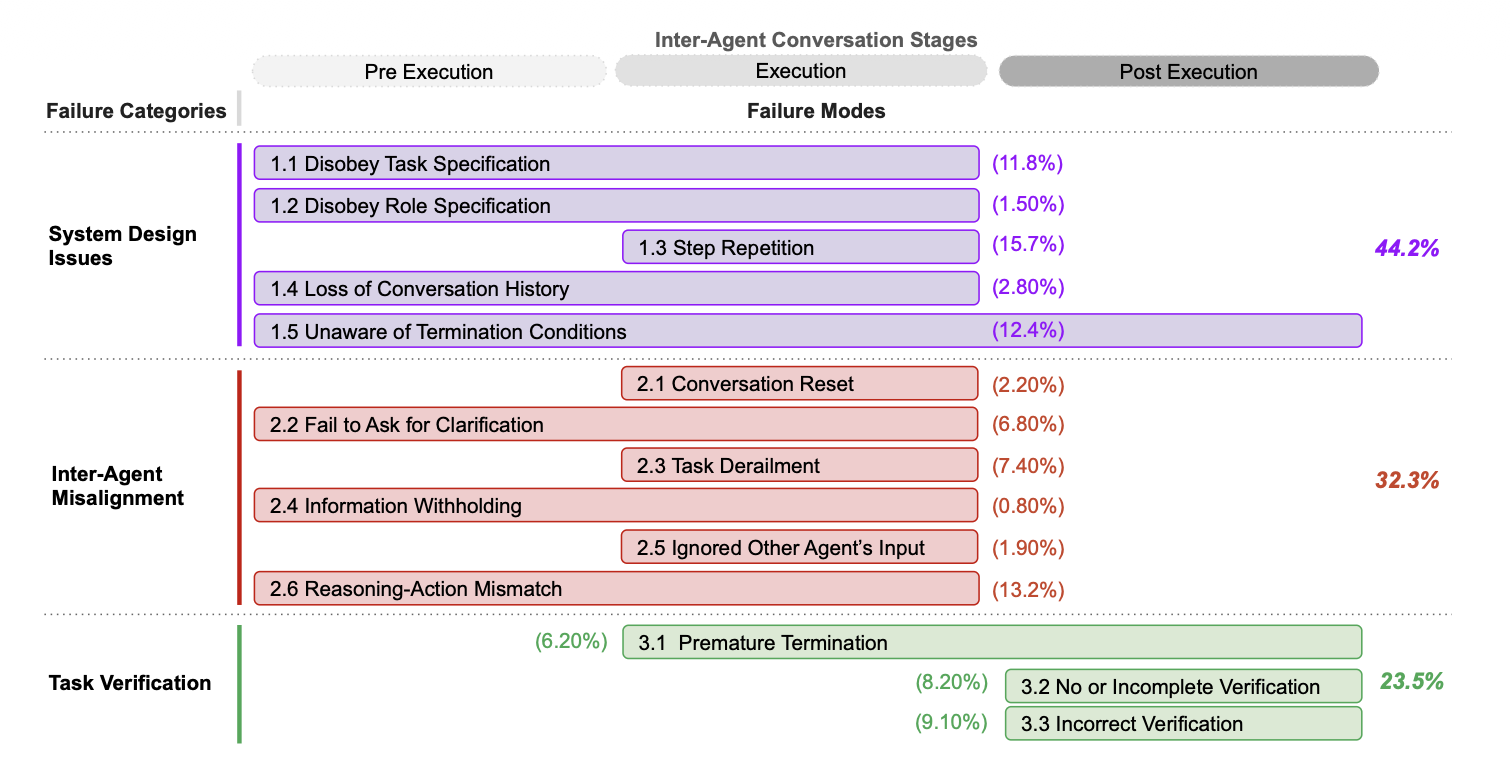
\includegraphics[keepaspectratio,alt={Taxonomie MAST des modes d\textquotesingle échec des systèmes multi-agents LLM. Source : Cemri et al. (2025).}]{images/taxomanie_MAST.png}}
\caption{Taxonomie MAST des modes d\textquotesingle échec des systèmes
multi-agents LLM. Source : Cemri et al. (2025).}
\end{figure}

Kapoor et al. (2024) ajoutent que la précision seule ne suffit pas à évaluer un agent : un système peut améliorer ses résultats par des stratégies de retry coûteuses, sans progrès scientifique ou organisationnel réel. Gao et al. (2025) montrent enfin que les gains des systèmes multi-agents diminuent lorsque les modèles de base deviennent plus performants, tandis que les coûts en tokens peuvent augmenter fortement.

Ces travaux convergent vers un même point : le multi-agent n'est pas une fin en soi. Une architecture multi-agents ne devient pertinente que si elle améliore simultanément la performance, le coût, la robustesse et la gouvernabilité. Les systèmes centralisés, où un superviseur ou un agent principal coordonne les autres par messages, peuvent créer des goulots d'étranglement, fragmenter le contexte et rendre les décisions difficiles à auditer. L'enjeu n'est donc pas de choisir abstraitement entre agent unique et multi-agent, mais d'identifier un mécanisme de coordination capable de réduire les coûts de communication, de rendre les traces inspectables et de conserver une forme d'adaptabilité.


\subsection{Pourquoi le probl\`eme est d\textquotesingle abord manag\'erial}

Les modes d\textquotesingle échec décrits jusqu\textquotesingle ici ne
sont pas réductibles à des défauts de modèles. Ils relèvent de la
coordination, de la gouvernance et du coût d\textquotesingle orchestration,
trois objets qui appartiennent à l\textquotesingle histoire longue des
sciences de gestion. Markus (1983), dans un article ancien mais devenu
canonique en \emph{Communications of the ACM}, établit que les échecs
d\textquotesingle implémentation des SI ne tiennent pas principalement
à des défauts techniques : ils apparaissent lorsque le système
redistribue le pouvoir et le contrôle au sein de
l\textquotesingle organisation (Markus, 1983, p. 430). Quatre décennies
plus tard, ce point reste opérant : passer d\textquotesingle une
coordination hiérarchique à une coordination assistée par GenAI
réalloue ce qui décide, ce qui est mesuré et ce
qu\textquotesingle on contrôle.

Le défi peut être résumé sous la forme d'une équation managériale. L'organisation veut bénéficier de l'autonomie des agents pour accélérer des tâches complexes, mais elle doit simultanément maîtriser les coûts d'orchestration, préserver la cohérence des systèmes existants, assurer la conformité, maintenir la responsabilité humaine et éviter une perte de contrôle sur les décisions collectives. Cette équation explique l'ordre du chapitre : avant de défendre une solution stigmergique, il faut d'abord préciser les conditions dans lesquelles une écologie agentique peut être considérée comme gouvernable.

\begin{table}[H]
\centering
\small
\begin{tabularx}{\linewidth}{@{}XXX@{}}
\toprule
\textbf{Problème observé} & \textbf{Risque organisationnel} & \textbf{Exigence de design} \\
\midrule
Productivité locale mais passage à l'échelle difficile & Gains non stabilisés au niveau organisationnel & Transformer l'usage individuel en capacité collective \\
Multiplication des agents et échanges de messages & Fragmentation du contexte, coût élevé, erreurs de coordination & Réduire les dépendances directes entre agents \\
Transformation de code legacy & Perte de sémantique métier, dette technique, risque opérationnel & Tracer chaque modification et valider automatiquement \\
Autonomie agentique & Dilution de responsabilité et confiance mal calibrée & Intégrer supervision humaine, auditabilité et points d'escalade \\
Évaluation centrée sur la précision & Optimisation coûteuse et peu robuste & Mesurer performance, coût, reproductibilité et conformité \\
\bottomrule
\end{tabularx}
\caption{Synthèse des tensions managériales repérées dans la littérature et exigences de design qui en découlent.}
\label{tab:rev-tensions-manageriales}
\end{table}

% =============================================================================
\section{Gouvernance, auditabilit\'e et conformit\'e dans les \'ecologies agentiques}\label{sec:rev-gouvernance}
% =============================================================================

Une écologie agentique ne peut être déployée en entreprise que si elle respecte un ensemble de contraintes qui précèdent le choix technique. Ces contraintes concernent la supervision humaine, l'auditabilité, la sécurité, l'alignement avec les normes internes et la conformité réglementaire. Elles sont particulièrement fortes dans les secteurs régulés, où la production logicielle touche des processus critiques et des données sensibles. Cette section établit donc les critères que toute solution d'orchestration doit satisfaire.

\subsection{Supervision humaine effective et design for oversight}\label{supervision-humaine-effective-et-design-for-oversight}

L'Article 14 de l'EU AI Act impose que les systèmes d'IA à haut risque soient conçus de manière à permettre une supervision humaine effective. Fink (2025) insiste sur le fait que cette supervision ne peut pas être purement symbolique : les humains doivent comprendre les capacités et limites du système, interpréter correctement les sorties, rester conscients du biais d'automation, pouvoir intervenir et pouvoir arrêter le système lorsque nécessaire. Holmström et al. (2023) distinguent plusieurs configurations de supervision : Human-in-the-loop, lorsque chaque décision exige une validation humaine ; Human-on-the-loop, lorsque le système agit avec surveillance humaine ; et Human-in-command, lorsque l'humain conserve un contrôle stratégique.

Pour les systèmes multi-agents appliqués à la transformation de code, le mode Human-on-the-loop apparaît particulièrement pertinent. Exiger une validation humaine à chaque micro-action rendrait l'automatisation peu utile ; à l'inverse, déléguer entièrement les transformations serait difficilement acceptable dans des environnements critiques. L'objectif est donc de permettre aux agents d'agir localement, tout en rendant leurs actions observables, interrompables et réversibles.

Santoni de Sio et van den Hoven (2018) fournissent un cadre complémentaire avec le Meaningful Human Control. Leur condition de tracking exige que le système reste sensible aux raisons et valeurs humaines pertinentes ; leur condition de tracing exige qu'il soit possible de relier les résultats du système à des humains responsables. Ces deux conditions sont décisives pour une coordination émergente : si les agents interagissent indirectement par des traces, ces traces doivent permettre de reconstituer les chaînes causales et les responsabilités.


\subsection{Guardrails et gouvernance par l'environnement}\label{guardrails-et-gouvernance-par-lenvironnement}

Grisold et al. (2025) introduisent le concept de guardrails pour les écologies humain-IA. Les guardrails désignent des zones de comportement désirable qui encadrent les opérations du système sans supprimer toute autonomie adaptative. Leur approche distingue des normes profondes, liées aux valeurs stables de l'organisation, et des normes de surface, plus opérationnelles et adaptables selon les contextes.

Cette distinction est importante pour l'orchestration agentique. Un agent peut être contraint par des règles inscrites dans son prompt, mais ces règles sont fragiles si elles ne sont pas matérialisées dans l'environnement. À l'inverse, un dépôt Git qui exige des commits signés, une pipeline CI/CD qui bloque un patch échouant aux tests, ou un système de tickets qui impose un lien entre modification et demande métier sont des guardrails environnementaux. Ils ne dépendent pas seulement de la bonne volonté de l'agent ; ils structurent l'espace d'action disponible.

Cette logique prépare directement l'intérêt de la stigmergie. Si les agents se coordonnent par un environnement partagé, cet environnement peut devenir à la fois médium de coordination et dispositif de gouvernance. Les traces laissées par les agents ne servent pas seulement à informer les autres agents ; elles servent aussi à auditer, filtrer, renforcer, corriger ou annuler des actions. La gouvernance n'est plus une couche externe, elle devient une propriété du médium.


\subsection{Perspective principal-agent}

Jarrahi et Ritala (2025), dans \emph{California Management Review},
mobilisent la théorie économique principal-agent pour décrire la
relation entre utilisateurs et agents IA. Leur point de départ est que
les agents IA agissent pour le compte de leurs utilisateurs dans un
périmètre défini, mais disposent d\textquotesingle une capacité de
traitement et d\textquotesingle un accès à l\textquotesingle information
supérieurs aux humains qu\textquotesingle ils servent (Jarrahi et
Ritala, 2025, p. 2) : on retrouve ici l\textquotesingle asymétrie
classique de la théorie de l\textquotesingle agence. Les auteurs en tirent cinq
dimensions de gouvernance (interactivité et adaptabilité, autonomie
guidée, intelligence collective, sécurité et responsabilité,
interopérabilité), à orchestrer, individualiser et aligner sur les
objectifs du principal. Les auteurs insistent sur la traçabilité des
décisions agents comme prérequis à toute \emph{accountability}
organisationnelle (Jarrahi et Ritala, 2025, p. 9) ; les systèmes de
contrôle de version, qui conservent par construction
l\textquotesingle historique des modifications, fournissent une
infrastructure naturelle pour cette exigence.

\begin{figure}[H]
\centering
\pandocbounded{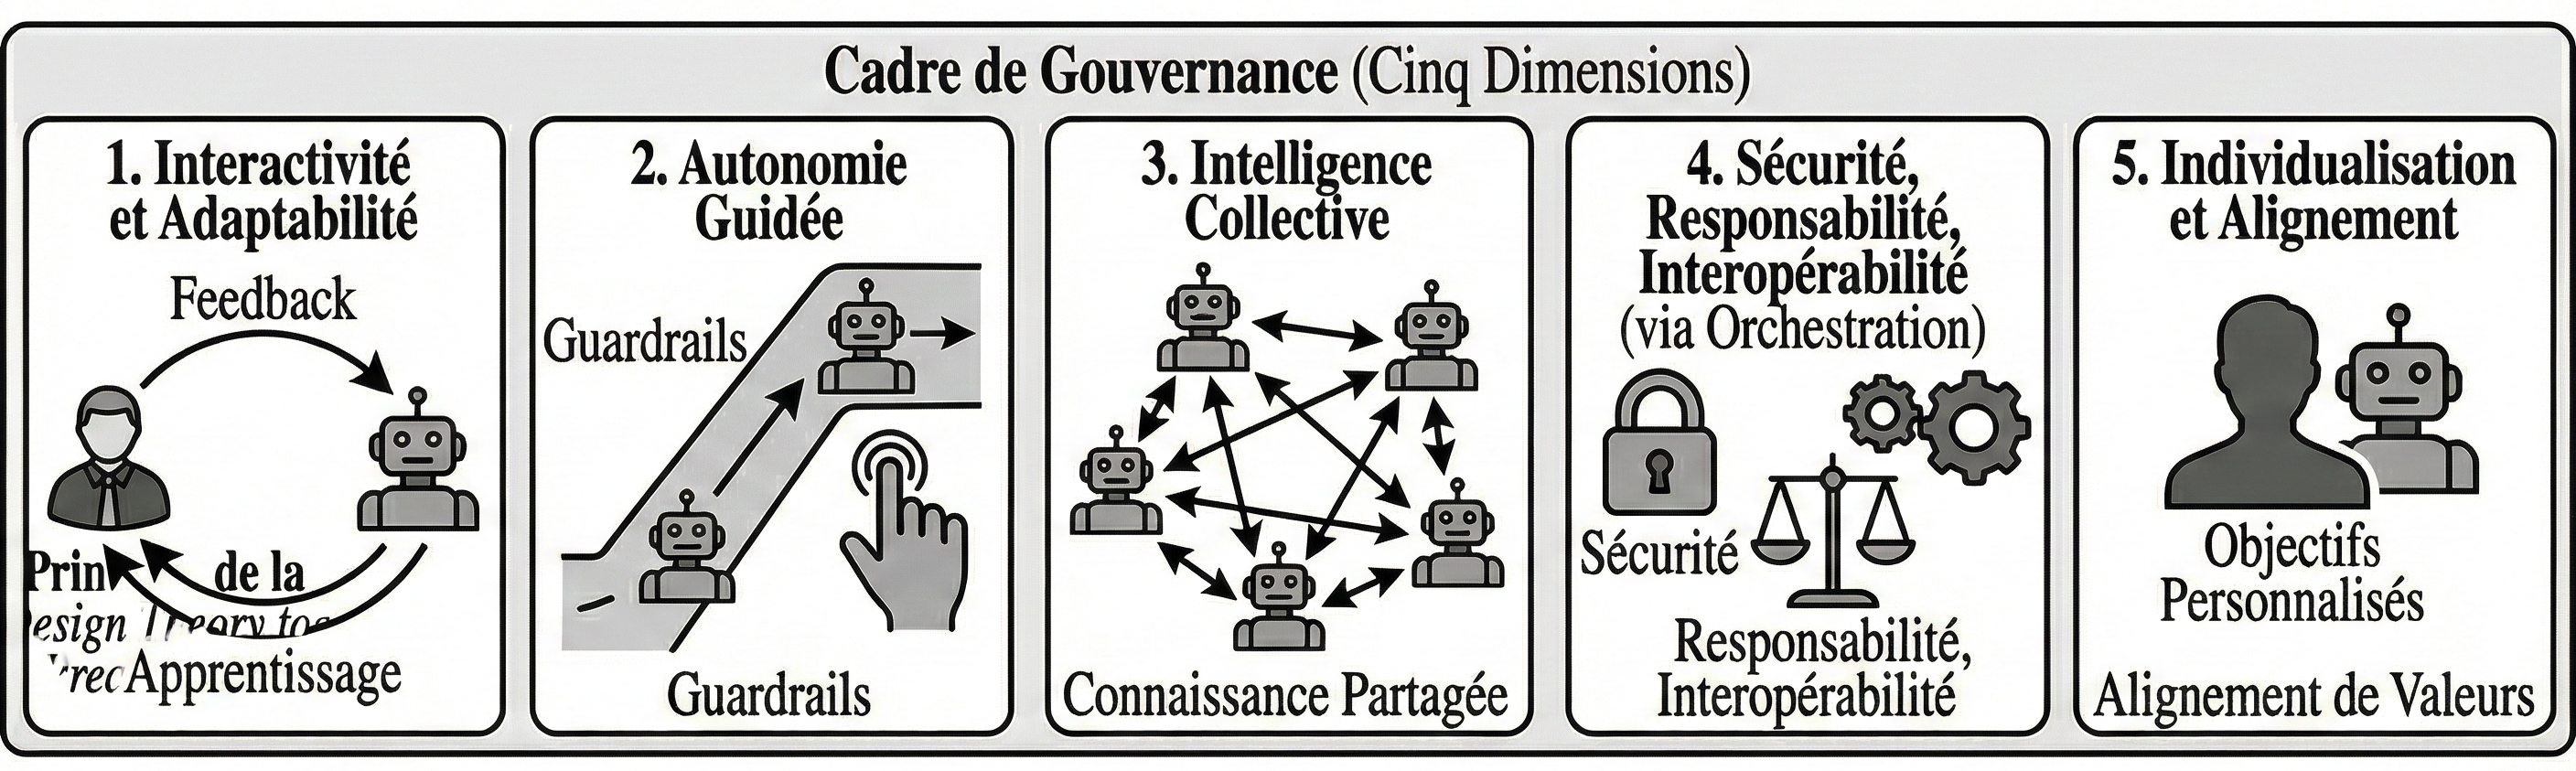
\includegraphics[keepaspectratio,alt={Cadre de gouvernance pour systèmes multi-agents : articulation des dimensions de contrôle, responsabilité et alignement. Source : adaptation de Jarrahi et Ritala (2025).}]{images/cadre_de_gouvernance.png}}
\caption{Cadre de gouvernance pour systèmes multi-agents : articulation
des dimensions de contrôle, responsabilité et alignement. Source :
adaptation de Jarrahi et Ritala (2025).}
\end{figure}

\subsection{Spécificité des secteurs régulés : banque, données et résilience opérationnelle}\label{spuxe9cificituxe9-des-secteurs-ruxe9guluxe9s-banque-donnuxe9es-et-ruxe9silience-opuxe9rationnelle}

Dans les secteurs régulés, les exigences précédentes sont renforcées par des cadres sectoriels. Le RGPD impose la maîtrise des traitements de données et la capacité à justifier certains usages ; le Digital Operational Resilience Act renforce les exigences de résilience numérique pour les institutions financières ; les autorités de supervision sectorielle exigent des dispositifs de contrôle adaptés aux risques opérationnels, aux données sensibles et aux processus critiques. Dans ce contexte, une écologie agentique appliquée au système d'information ne peut pas fonctionner comme une boîte noire expérimentale.

La banque constitue donc un terrain particulièrement exigeant. Les systèmes y sont souvent anciens, interconnectés et soumis à des contraintes fortes de disponibilité. Une erreur de transformation logicielle peut avoir des effets opérationnels, juridiques et réputationnels. Cela justifie de privilégier des mécanismes d'audit append-only, des journaux d'exécution exploitables par les fonctions de contrôle, des validations automatiques reproductibles et des points de décision humaine clairement définis. La solution technique doit être pensée dès l'origine comme compatible avec l'audit interne, la conformité et la continuité d'activité.


\subsection{Articulation gouvernance externe et gouvernance interne}

Respecter les textes ne suffit pas : encore faut-il que les exigences
externes se traduisent en politiques opérationnelles applicables au
quotidien. Cette traduction est portée par la DSI, par les comités IA
internes et par les fonctions d\textquotesingle audit et de conformité.
Pour qu\textquotesingle elle aboutisse, les artefacts produits par les
agents (issues, commits, logs, métriques) doivent rester directement
lisibles par les opérateurs humains, et pas seulement consommables par
des outils techniques. À défaut, la gouvernance interne n\textquotesingle a
pas prise sur le système.

\subsection{Responsabilit\'e morale distribu\'ee et gouvernance \'ethique des syst\`emes swarm}

Floridi (2016) introduit dans \emph{Philosophical Transactions of the
Royal Society A} le concept de \emph{Distributed Moral Actions} (DMAs) :
des actions moralement significatives qui résultent
d\textquotesingle interactions locales individuellement neutres. Cette
notion permet de décrire comment des comportements émergents à portée
morale peuvent surgir d\textquotesingle interactions stigmergiques
individuellement banales. Winfield et al. (2025), dans la même revue,
observent un retournement intéressant : dans les systèmes
conventionnels, une propriété émergente est un \emph{bug} à corriger,
alors que dans les systèmes \emph{swarm}, c\textquotesingle est une
propriété recherchée. La conséquence en termes de gouvernance est nette :
les comportements émergents des orchestrations stigmergiques doivent
être gouvernés, pas supprimés, ce qui suppose des cadres distincts de
l\textquotesingle assurance qualité traditionnelle. Mukherjee et Chang
(2025) proposent dans cette direction le framework
\emph{Operational Agency}, qui trace l\textquotesingle intention et la
responsabilité dans les systèmes multi-agents IA et donne un mécanisme
de reconstruction causale des décisions collectives.

García-Ruiz et Rocchi (2025) ajoutent une dimension éthique à ce
diagnostic. En s\textquotesingle appuyant sur la philosophie des vertus
d\textquotesingle Alasdair MacIntyre, ils défendent que le travail
significatif suppose l\textquotesingle exercice d\textquotesingle une
agentivité morale, c\textquotesingle est-à-dire la capacité de prendre
des décisions délibérées qui reflètent des valeurs et un jugement
professionnel. Le management algorithmique, lorsqu\textquotesingle il
réduit le rôle humain à valider mécaniquement des prescriptions
automatisées, érode cette agentivité et appauvrit la portée du travail.
La conséquence pour l\textquotesingle orchestration agentique en
entreprise est claire : la conformité réglementaire ne suffit pas à
justifier un déploiement. Il faut prévoir des points
d\textquotesingle intervention humaine où le jugement a une portée
réelle, et non simplement des cases à cocher pour faire valider une
décision déjà prise par les agents.

\subsection{S\'ecurit\'e des syst\`emes multi-agents}

Chen et al. (2024), dans un article publié à NeurIPS 2024, documentent
\emph{AgentPoison}, première attaque \emph{backdoor} ciblant les bases
de connaissances RAG et les mémoires persistantes des agents LLM, avec
un taux de succès d\textquotesingle au moins 80 \% pour un taux de
poison inférieur à 0,1 \%. L\textquotesingle environnement partagé,
équivalent stigmergique aux phéromones numériques, devient un vecteur
d\textquotesingle attaque persistante créant une vulnérabilité
spécifique aux architectures de coordination indirecte. Lee et Tiwari
(2024) documentent le \emph{Prompt Infection}, injection de prompts
LLM-to-LLM se propageant silencieusement entre agents interconnectés,
l\textquotesingle analogie virale est ici directement opérante pour des
systèmes de coordination indirecte. Ces vulnérabilités imposent des exigences de
sécurité spécifiques pour les orchestrations stigmergiques :
authentification des traces déposées dans l\textquotesingle environnement,
validation de l\textquotesingle intégrité des artefacts partagés et
mécanismes de détection d\textquotesingle anomalies dans les patterns de
coordination émergents.

Mises bout à bout, ces contraintes (réglementaires, sectorielles,
organisationnelles, éthiques, sécuritaires) convergent vers une même
conclusion : une orchestration agentique en entreprise n\textquotesingle est
viable que si la gouvernance est intégrée dès la conception. Tenter de
l\textquotesingle ajouter après coup conduit aux échecs documentés en
\S\ref{sec:rev-defi-managerial}. C\textquotesingle est cette contrainte
qui borne le reste de la revue.


La gouvernance des écologies agentiques impose une conclusion claire : le système de coordination doit être en même temps un système d'audit. Les agents doivent pouvoir agir, mais leurs actions doivent laisser des traces interprétables ; les humains doivent pouvoir superviser, mais sans bloquer chaque micro-action ; les règles doivent encadrer le comportement, mais sans supprimer toute adaptation. Ces exigences orientent la revue vers les théories de la coordination organisationnelle, car il faut désormais comprendre comment des activités interdépendantes peuvent être organisées sans dépendre d'un superviseur central omniscient.

% =============================================================================
\section{Th\'eorie de la coordination organisationnelle et apport au management des SI}\label{sec:rev-coordination-org}
% =============================================================================

La littérature sur les agents LLM emploie souvent le terme d'orchestration dans un sens technique : organiser des appels de modèles, répartir des tâches ou définir une topologie d'échanges. Pour un mémoire en management des systèmes d'information, cette notion doit être replacée dans une théorie plus générale de la coordination. Une écologie agentique est un système organisationnel : elle gère des dépendances entre activités, distribue des rôles, produit des artefacts, actualise des routines et transforme des capacités.

\subsection{Th\'eorie de la coordination (Malone et Crowston, 1994)}

Malone et Crowston (1994), dans un article fondateur publié dans
\emph{ACM Computing Surveys}, définissent la coordination comme la
gestion des dépendances entre activités. Leur taxonomie identifie
plusieurs mécanismes selon le type de dépendance, les hiérarchies gèrent
les dépendances par autorité centralisée, les marchés par ajustement de
prix, et la communication directe par échanges de messages entre
acteurs. La stigmergie constitue un quatrième mécanisme, très peu
identifié dans la littérature managériale mais formellement cohérent
avec leur cadre : elle gère les dépendances par modification
environnementale, les agents se coordonnant en lisant et en écrivant
dans un artefact partagé plutôt que par messages directs ou par
soumission à une autorité centrale.

Situer la stigmergie dans le vocabulaire des sciences de gestion change
le statut de l\textquotesingle objet : ce n\textquotesingle est plus
une curiosité biologique transposée à
l\textquotesingle informatique, c\textquotesingle est un mécanisme de
coordination organisationnel comparable, dans le même cadre formel, aux
hiérarchies, aux marchés et à la communication directe. Bolici et al.
(2016) ont d\textquotesingle ailleurs vérifié empiriquement
la présence de ce mécanisme dans les équipes de développement open
source distribuées, ce qui ancre empiriquement la transposition du
concept aux organisations logicielles au-delà du seul argument
théorique. Du
point de vue de la coordination, l\textquotesingle intérêt analytique
est tangible : la communication indirecte réduit le nombre de liens de
$O(n^2)$ à $O(n)$, supprime les goulots
d\textquotesingle étranglement centraux et permet de découpler
temporellement des activités interdépendantes.

\subsection{Capacit\'es dynamiques et orchestration strat\'egique (Teece, 2007)}

Teece (2007) définit les capacités dynamiques comme l'aptitude d'une organisation à détecter les opportunités et menaces, à saisir les occasions, puis à reconfigurer ses actifs pour maintenir un avantage compétitif. La transformation logicielle peut être relue à travers ce cadre. Moderniser un système, migrer une version de langage, réduire une dette technique ou adapter une architecture ne sont pas de simples tâches de maintenance ; ce sont des opérations par lesquelles l'organisation maintient sa capacité à évoluer.

L'IA agentique devient pertinente si elle renforce cette capacité dynamique. Des agents peuvent détecter des zones de dette technique, proposer des modifications, tester des variantes, documenter des changements et accélérer la reconfiguration d'actifs logiciels. Mais cette capacité n'a de valeur que si elle est maîtrisée. Une transformation rapide mais non traçable ou non gouvernable peut augmenter le risque. L'orchestration attendue doit donc permettre une reconfiguration continue, mais contrôlée.

Cette lecture rapproche le travail technique du management stratégique. L'artefact logiciel n'est pas seulement un outil ; il est un actif organisationnel. L'agent LLM n'est pas seulement un générateur ; il devient une ressource d'orchestration. Le manager SI n'est pas seulement un superviseur de projet ; il doit définir les conditions dans lesquelles cette orchestration contribue à la capacité dynamique de l'organisation.


\subsection{Routines organisationnelles et \'evolution du code (Feldman et Pentland, 2003)}

Feldman et Pentland (2003), dans un article influent publié dans
\emph{Administrative Science Quarterly}, reconceptualisent les routines
organisationnelles non comme des structures statiques mais comme des
sources de flexibilité et de changement. Ils distinguent
l\textquotesingle aspect ostensif (la structure abstraite de la routine
telle que comprise par les acteurs) et l\textquotesingle aspect
performatif (les actions concrètes réalisées par des personnes
spécifiques à des moments spécifiques). Les routines évoluent par
l\textquotesingle interaction continue entre ces deux aspects.

Cette grille s\textquotesingle applique directement à la transformation
de code vue comme processus organisationnel. Le code source incarne des
routines : chaque fonction, chaque module encode des procédures, des
règles métier et des pratiques qui structurent
l\textquotesingle activité courante. Transformer du code, ce
n\textquotesingle est donc pas une opération neutre : c\textquotesingle est
toucher à des routines, avec ce que cela implique en termes de
résistance, de perte de savoir tacite et de recomposition des pratiques.
Une coordination stigmergique préserve l\textquotesingle aspect ostensif
(les agents respectent la structure du code en place comme contexte) et
laisse évoluer l\textquotesingle aspect performatif (les transformations
restent incrémentales et traçables). Les traces déposées dans
l\textquotesingle environnement, commits, métadonnées, résultats de
tests, constituent la mémoire organisationnelle de cette évolution et
rendent possibles l\textquotesingle audit, l\textquotesingle apprentissage
et la réversibilité.

\subsection{Affordances technologiques (Strong et al., 2014)}

Strong et al. (2014) définissent les affordances technologiques comme des possibilités d'action offertes par une technologie à des acteurs situés. Une même technologie peut donc produire des effets différents selon les acteurs, les objectifs, les routines et les contraintes organisationnelles. Cette notion est utile pour éviter un déterminisme technologique : l'IA agentique ne crée pas mécaniquement de valeur ; elle offre des possibilités qui doivent être actualisées dans un contexte.

Les affordances pertinentes pour cette recherche sont notamment la génération de modifications, la localisation de dépendances, la validation automatisée, la documentation, la coordination asynchrone, la traçabilité et l'escalade humaine. Le design de l'artefact doit rendre ces affordances actualisables. Par exemple, un agent capable de générer un patch ne crée de valeur que si le patch peut être relié à une tâche, testé, comparé, revu et intégré dans une chaîne de gouvernance.

L'approche par affordances relie donc directement le choix technique à la valeur managériale. Une architecture stigmergique n'est pertinente que si elle permet aux acteurs organisationnels d'actualiser des possibilités que les architectures centralisées ou purement conversationnelles actualisent mal : coordination asynchrone, auditabilité native, réduction de la charge de supervision et apprentissage à partir des traces.

\subsection{D\'efinitions op\'eratoires : agent LLM, syst\`eme multi-agent, orchestration}

Afin de stabiliser le vocabulaire, cette recherche retient quatre définitions opératoires. Un agent LLM est un composant logiciel fondé sur un modèle de langage, capable d'interpréter un objectif, de produire un raisonnement ou une action, d'utiliser des outils et de modifier ou consulter des artefacts. Un système multi-agents LLM est un ensemble de plusieurs agents spécialisés ou redondants qui contribuent à un objectif commun ou à des objectifs interdépendants. Une orchestration désigne l'organisation des rôles, des dépendances, des règles d'action, des mécanismes de validation et des flux d'information entre ces agents. Enfin, un médium de coordination désigne l'environnement partagé par lequel les agents observent l'état du travail, déposent des traces et déclenchent des actions ultérieures.

Ces définitions permettent de distinguer l'objet de recherche d'un simple chatbot ou d'un pipeline linéaire. Le coeur du problème n'est pas la génération isolée d'une sortie, mais l'organisation d'un collectif agentique dans le temps. C'est à ce niveau que la stigmergie devient une piste théorique et opérationnelle.

\begin{figure}[H]
\centering
\pandocbounded{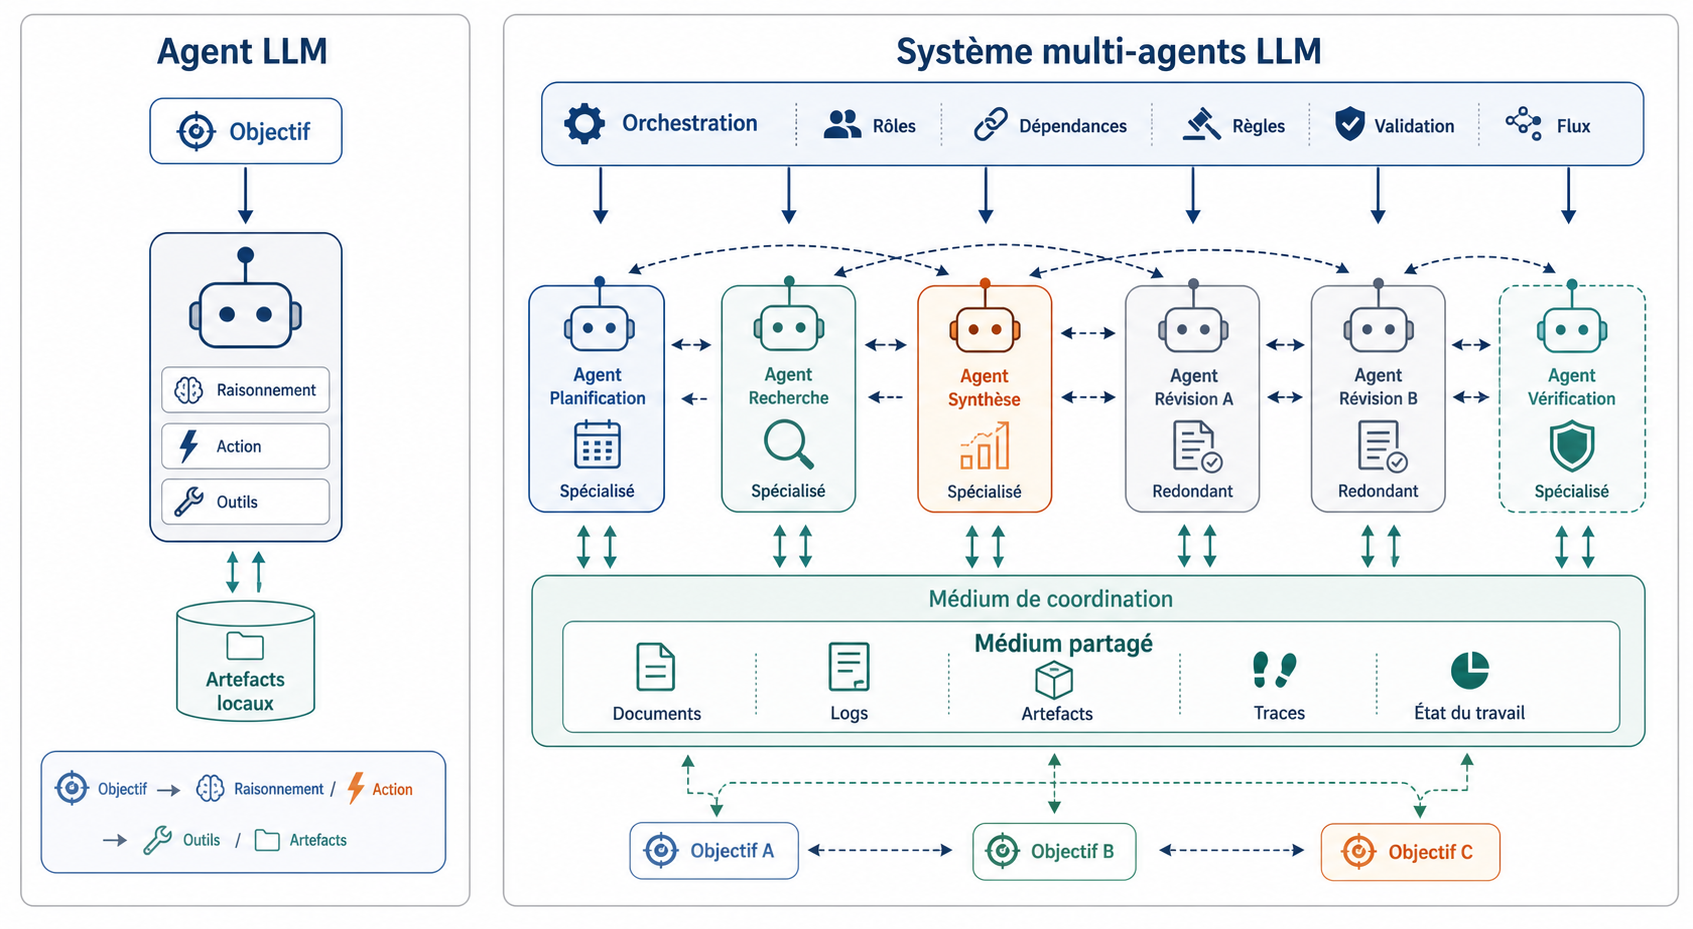
\includegraphics[keepaspectratio,alt={Agent LLM vs système multi-agent (MAS) : comparaison des niveaux d\textquotesingle organisation et des modes de coordination. Source : adaptation de Cemri et al. (2025) et Gao et al. (2025).}]{images/definitions_operatoires_direct.png}}
\caption{Agent LLM versus système multi-agent (MAS) : comparaison des
niveaux d\textquotesingle organisation et des modes de coordination.
Source : adaptation de Cemri et al. (2025) et Gao et al. (2025).}
\end{figure}


% =============================================================================
\section{La stigmergie comme m\'ecanisme de coordination indirecte}\label{sec:rev-stigmergie}
% =============================================================================

La stigmergie est souvent présentée à partir de son origine biologique. Pour cette recherche, son intérêt principal n'est pas la métaphore de la fourmi ou du termite, mais le principe abstrait qu'elle révèle : des acteurs peuvent se coordonner indirectement en modifiant un environnement commun. L'environnement conserve des traces de l'activité passée ; ces traces influencent l'activité future ; la coordination collective émerge sans qu'un superviseur central doive prescrire chaque action.


\subsection{Origine biologique et formalisation algorithmique}

Le terme « stigmergie » fut introduit par Pierre-Paul Grassé dans son
étude des comportements de construction chez les termites (Grassé,
1959). Grassé observa un paradoxe fondamental, les termites semblaient
travailler indépendamment tout en produisant des structures
collectivement cohérentes, et le résolut en identifiant un mécanisme
tiers, la coordination indirecte médiée par
l\textquotesingle environnement. Le néologisme combine les racines
grecques \emph{stigma} (marque) et \emph{ergon} (travail) : la
stimulation des ouvriers par les performances qu\textquotesingle ils ont
eux-mêmes accomplies (Grassé, 1959). 
La formalisation algorithmique de la stigmergie repose généralement sur trois mécanismes : le dépôt de traces, le renforcement des traces utiles et l'évaporation ou la disparition progressive des traces moins utiles. Dans les algorithmes inspirés des colonies de fourmis, ces traces sont souvent modélisées comme des phéromones qui orientent la recherche de chemins. L'intérêt pour les systèmes d'information est double. D'une part, la coordination ne dépend pas d'une communication directe entre tous les acteurs. D'autre part, le système peut s'adapter dynamiquement, car les traces évoluent avec l'activité réelle.

\begin{figure}[H]
\centering
\pandocbounded{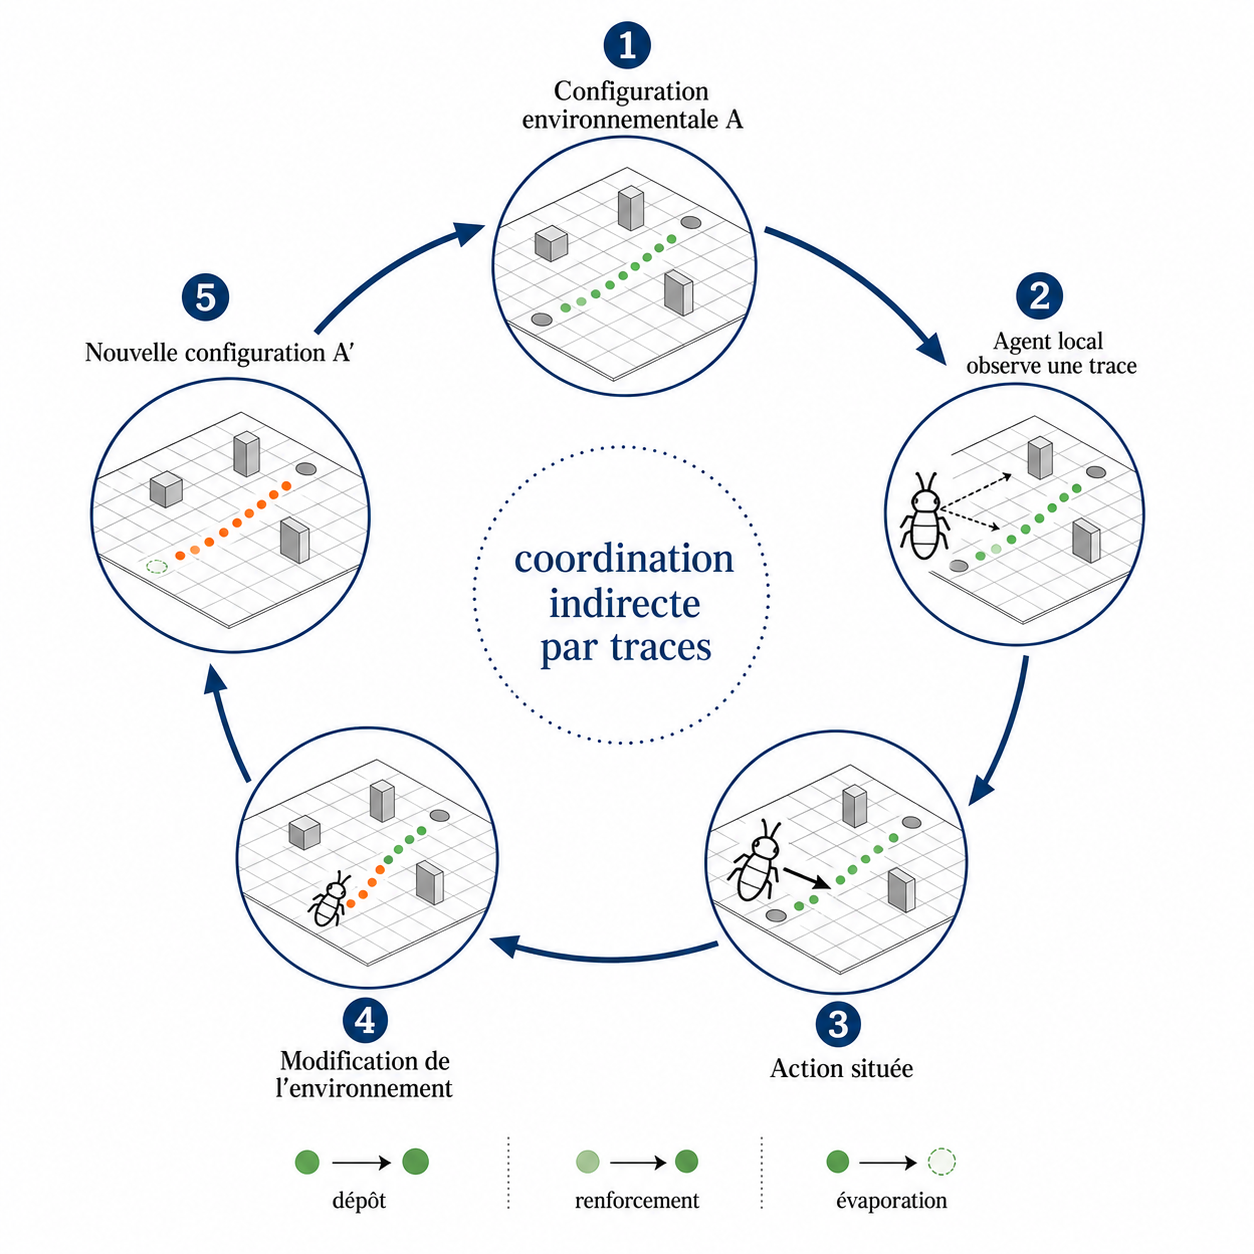
\includegraphics[width=0.75\linewidth,keepaspectratio,alt={Boucle de rétroaction stigmergique : une action modifie l\textquotesingle environnement, ce qui déclenche l\textquotesingle action suivante. Source : adaptation à partir de Grassé (1959) et Bonabeau et al. (1999).}]{images/stigmergic_feedback_loop_direct_fr_academic.png}}
\caption{Boucle de rétroaction stigmergique : une action modifie
l\textquotesingle environnement, ce qui déclenche
l\textquotesingle action suivante. Source : adaptation à partir de
Grassé (1959) et Bonabeau et al. (1999).}
\end{figure}

L\textquotesingle ouvrage \emph{Swarm Intelligence: From Natural to
Artificial Systems} (Bonabeau et al., 1999) établit
l\textquotesingle intelligence en essaim comme discipline scientifique,
et articule le rôle de la modélisation comme interface entre
compréhension de la nature et conception de systèmes artificiels
(Bonabeau et al., 1999, p. 18). Theraulaz et Bonabeau (1999)
distinguent deux modalités fondamentales, la stigmergie quantitative,
où l\textquotesingle intensité de la trace affecte la probabilité
d\textquotesingle une action, et la stigmergie qualitative, où des
stimuli qualitativement différents déclenchent des réponses
qualitativement différentes (Theraulaz et Bonabeau, 1999, p.
104-105). Cette typologie fournit un vocabulaire pour guider le choix
entre approches de coordination dans la conception de systèmes
multi-agents.

\begin{figure}[H]
\centering
\pandocbounded{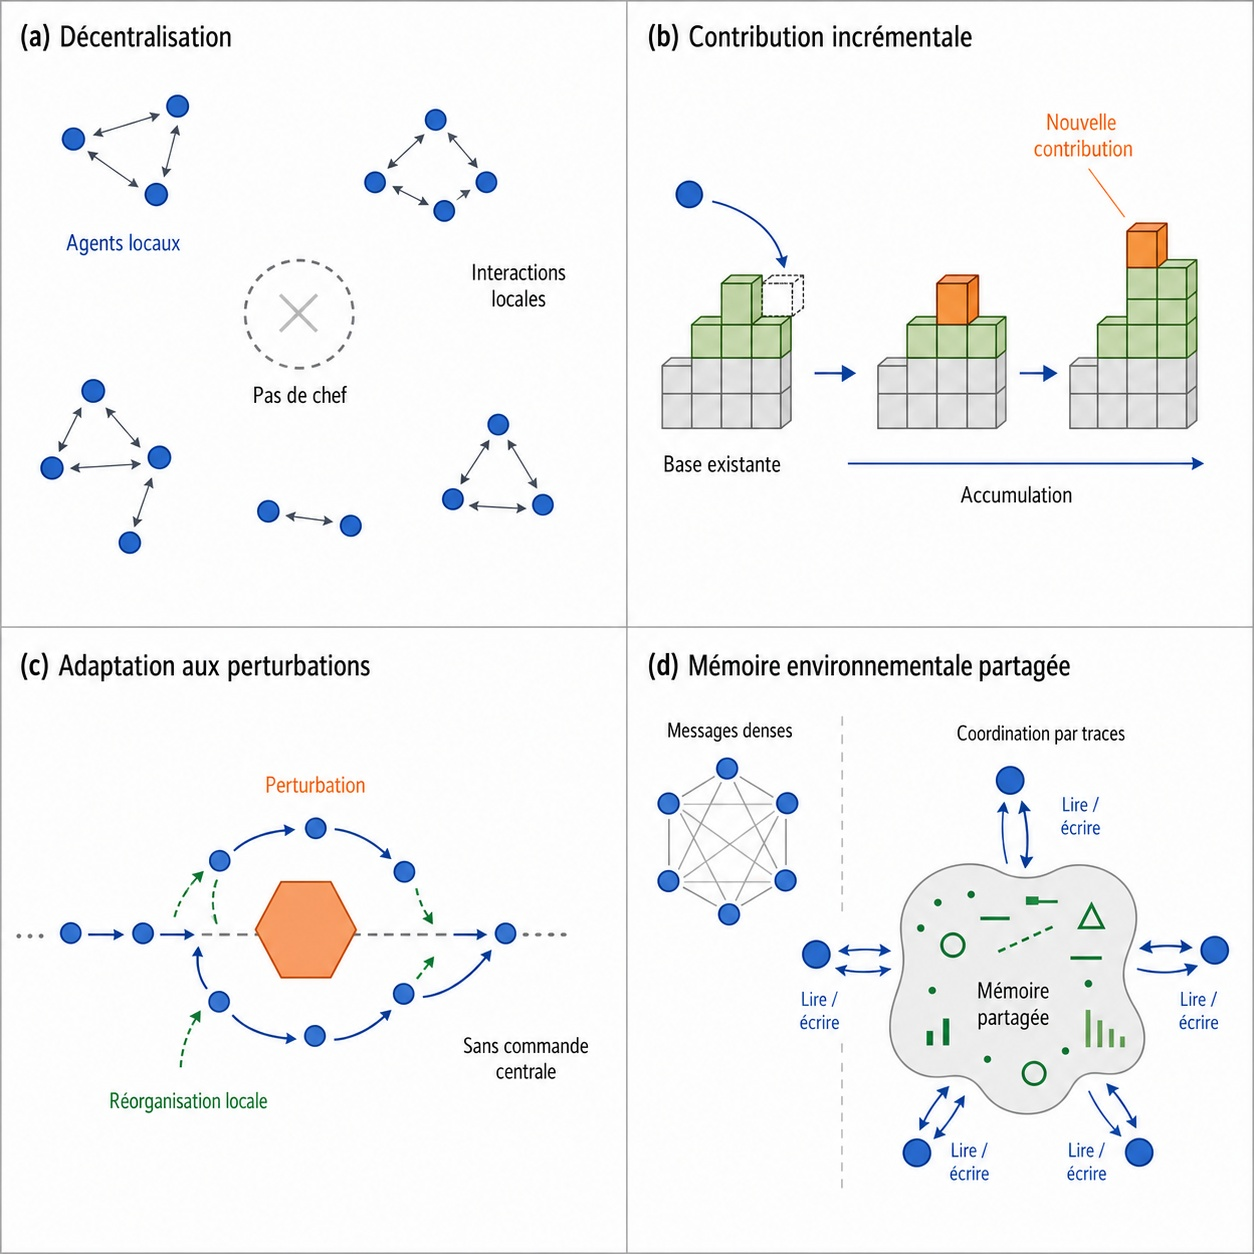
\includegraphics[width=0.74\linewidth,keepaspectratio,alt={Principes fondamentaux des systèmes auto-organisés : décentralisation, contribution incrémentale, adaptation et mémoire environnementale partagée. Source : Bonabeau et al. (1999) ; Marsh et Onof (2008).}]{images/self_organizing_principles_paperbanana_auto_ref40_filtered_fr_academic.png}}
\caption{Principes fondamentaux des systèmes auto-organisés :
décentralisation, contribution incrémentale, adaptation et mémoire
environnementale partagée. Source : Bonabeau et al. (1999) ; Marsh et
Onof (2008).}
\end{figure}

\subsection{Extension num\'erique : Heylighen et la stigmergie comme m\'ecanisme universel}

Heylighen (2016a, 2016b) propose la première formalisation générale de
la stigmergie. Sa définition est sobre : la stigmergie est le mécanisme
de coordination indirecte par lequel la trace qu\textquotesingle une
action laisse dans un médium stimule les actions suivantes (Heylighen,
2016a). Heylighen (2016b) raffine la typologie en
distinguant la stigmergie sématectonique, où la stimulation provient
directement du travail accompli sur l\textquotesingle environnement,
et la stigmergie basée sur marqueurs, où des signaux dédiés rendent
saillantes des traces qui ne contribuent pas elles-mêmes à la tâche. En
contexte numérique, l\textquotesingle exemple parlant est Wikipédia :
les contributeurs réagissent soit aux lacunes visibles du texte
(sématectonique), soit aux balises explicites « à faire » apposées dans
les pages (marqueurs) (Heylighen, 2016b, p. 51). L\textquotesingle apport
de fond de Heylighen est d\textquotesingle identifier la stigmergie
comme mécanisme commun à Wikipédia, au développement open source, aux
systèmes de contrôle de version et même au mécanisme de prix
(Heylighen, 2016a). Vue sous cet angle, la stigmergie n\textquotesingle est
pas une curiosité importée de la biologie : c\textquotesingle est une
forme générale de coordination dans les écosystèmes humains et
numériques.

Cette généralisation prolonge un travail amorcé plus tôt par Parunak
(1997), qui formule des principes d\textquotesingle ingénierie pour les
systèmes multi-agents directement inspirés des collectifs naturels :
localité de la perception et de l\textquotesingle action, coordination
par traces, feedback positif, redondance et adaptation collective. Sa
thèse architecturale est qu\textquotesingle un système robuste ne tient
pas à la sophistication individuelle de ses composants mais à la
diversité des interactions locales qu\textquotesingle ils peuvent
entretenir avec un environnement partagé. C\textquotesingle est ce
déplacement, formalisé chez Heylighen, qui rend la stigmergie
opératoire pour des systèmes d\textquotesingle information.

\subsection{Développements récents bio-inspirés et prudence conceptuelle}\label{duxe9veloppements-ruxe9cents-bio-inspiruxe9s-et-prudence-conceptuelle}

Plusieurs travaux récents réintroduisent explicitement des mécanismes bio-inspirés dans l'orchestration agentique. Chari et al.~(2025) proposent par exemple une approche combinant modèles de langage et logique de phéromones pour apprendre des chemins de raisonnement. Zhang et al.~(2025), avec SwarmAgentic, explorent la génération de systèmes agentiques via des principes inspirés de l'intelligence en essaim. Rodriguez (2026) formalise une coordination par champs de pression et décroissance temporelle. Ces travaux indiquent un intérêt croissant pour des formes de coordination émergente au-delà des architectures conversationnelles classiques.

Il faut cependant rester prudent. Rahman et al.~(2025) soulignent que le terme swarm peut être conceptuellement extensible lorsqu'il est appliqué à des agents LLM. Les agents biologiques simples ne sont pas équivalents à des agents fondés sur des modèles de langage, capables de raisonner, de manipuler des symboles et d'interagir avec des outils complexes. C'est pourquoi la présente recherche ne se fonde pas sur une transposition naïve de l'intelligence en essaim. Elle privilégie la stigmergie cognitive, plus adaptée à des agents capables d'interpréter des artefacts et d'agir dans des environnements organisationnels.



\subsection{Panorama synth\'etique des frameworks}

Deux familles de frameworks coexistent pour concevoir des systèmes
multi-agents. D\textquotesingle un côté, les plateformes MAS classiques
pré-LLM (JADE, Jason, SPADE) reposent sur le \emph{message-passing} et
sur des modèles organisationnels explicites. De l\textquotesingle autre,
les frameworks LLM-natifs (LangGraph, AutoGen, CrewAI, MetaGPT)
orchestrent des agents LLM en intégrant directement le \emph{tool-use},
la gestion d\textquotesingle état et les topologies
d\textquotesingle interaction (Geng et Chang, 2025 ; Cemri et al.,
2025). MetaGPT formalise des \emph{Standardized Operating Procedures}
pour réduire les incohérences des chaînes d\textquotesingle agents en
génie logiciel (Hong et al., 2024). OpenHands propose une plateforme
open source pour développer et évaluer des agents généralistes en prise
sur dépôts, shell et tests (Wang et al., 2025). Ces frameworks sont utiles, mais ils ne résolvent pas entièrement le problème identifié plus haut. Beaucoup restent centrés sur la conversation, la séquence d'appels ou le contrôle par superviseur. Ils intègrent des outils et de la mémoire, mais rarement un médium stigmergique conçu comme système de coordination, d'audit et de gouvernance par construction. Le manque ne se situe donc pas dans l'absence d'agents ou d'outils, mais dans l'absence d'un principe de design unifié reliant coordination indirecte, traces, conformité et évaluation coût-performance.


La stigmergie fournit une réponse conceptuelle au problème posé en 2.1 et borné en 2.2. Elle permet d'envisager une coordination sans superviseur central omniscient, tout en conservant des traces exploitables. Sa version cognitive, fondée sur les agents et les artefacts, est compatible avec des agents LLM. Le développement logiciel offre déjà un substrat stigmergique, ce qui rend l'approche praticable. La section suivante examine donc le terrain où cette approche peut être testée de manière rigoureuse : la transformation de code.

% =============================================================================
\section{Transformation de code et workflows agentiques en pratique}\label{sec:rev-transformation-code}
% =============================================================================

La transformation de code constitue un terrain d'application pertinent pour trois raisons. Premièrement, elle est économiquement et stratégiquement importante pour les organisations confrontées à la modernisation de leurs systèmes. Deuxièmement, elle combine des tâches adaptées aux agents LLM - compréhension de code, génération de patches, documentation, analyse de logs - avec des contraintes fortes de validation. Troisièmement, elle produit naturellement des traces : diffs, commits, tests, tickets, métriques et revues. Elle permet donc d'évaluer concrètement une orchestration stigmergique.

\subsection{Validation industrielle \`a grande \'echelle}

Ziftci et al.~(2025) documentent une migration de code assistée par LLM à grande échelle chez Google. Leur approche combine analyse statique, génération de modifications, validation automatisée et revue humaine sélective. Les résultats montrent qu'une partie importante des changements peut être appliquée sans modification humaine, tout en réduisant le temps développeur. Mais les auteurs identifient aussi des limites : fenêtre de contexte, tests existants insuffisants, cas complexes nécessitant une intervention humaine et dépendance à la qualité des artefacts d'entrée.

Ces observations sont directement utiles pour cette recherche. Elles montrent que les LLM peuvent contribuer à la transformation de code, mais que leur valeur dépend d'un système de coordination plus large. Un patch généré n'est qu'une étape ; il doit être localisé, expliqué, testé, comparé, éventuellement corrigé, puis intégré. L'architecture d'orchestration doit donc coordonner des activités multiples et laisser des traces exploitables à chaque étape.

Les cas industriels autour de la modernisation legacy, notamment les migrations COBOL vers Java ou les évolutions d'écosystèmes Java, confirment la réalité du besoin. Sneed (2010) montre la difficulté structurelle des migrations legacy. IBM (2023) et Amazon (2024) illustrent l'intérêt industriel pour l'automatisation de la modernisation applicative. Diggs et al.~(2025) soulignent également l'importance de la documentation générée par LLM pour comprendre du code ancien avant transformation. Ces travaux convergent : le problème n'est pas seulement de produire du code nouveau, mais de transformer du code existant en conservant sa signification.

\subsection{Traduction cross-langage et \'evolution d\textquotesingle API}

Rozière et al.~(2020) montrent que la traduction non supervisée entre langages de programmation peut atteindre des performances significatives grâce à des techniques de back-translation et de denoising auto-encoding. CodeRosetta (2024) prolonge cette logique vers la programmation parallèle. Ces travaux indiquent que les modèles peuvent apprendre des correspondances entre langages et produire des traductions plausibles.

Cependant, la transformation de code ne se réduit pas à une traduction syntaxique. Lamothe, Guéhéneuc et Shang (2021) montrent, dans leur revue systématique, que l'évolution des API est un problème central du génie logiciel. Les breaking changes, les dépendances obsolètes, les comportements implicites et les différences de sémantique exigent une compréhension contextuelle. Dig et Johnson (2005) soulignent que les refactorings jouent un rôle important dans l'évolution des API et peuvent servir de base à des outils de migration automatisée.

Pour un système multi-agents, ces travaux impliquent une division du travail possible : un agent peut localiser les usages d'une API, un autre proposer un mapping de migration, un autre générer le patch, un autre exécuter les tests, un autre analyser les erreurs. Mais cette division du travail n'est utile que si elle est coordonnée par des artefacts partagés. Sinon, les agents risquent de produire des corrections contradictoires, de perdre le contexte ou de répéter des erreurs déjà identifiées.

\subsection{De l\textquotesingle automatisation des processus \`a l\textquotesingle Agentic BPM}

La transformation de code s'inscrit dans une évolution plus large de l'automatisation des processus. Les approches RPA traditionnelles automatisent des tâches déterministes et répétitives. L'automatisation cognitive ajoute des capacités de perception, de classification ou de génération. L'Agentic Business Process Management pousse plus loin cette évolution en introduisant des agents capables d'agir de manière plus autonome dans des processus métier.

Vu et al.~(2026) proposent une conceptualisation de l'Agentic BPM qui distingue les agents pour le BPM et le BPM pour les agents. La première perspective utilise des agents pour exécuter ou améliorer des processus ; la seconde applique les principes du BPM pour gouverner les agents eux-mêmes. Dumas et al.~(2026) décrivent les Agentic BPMS comme des systèmes où les flux ne sont pas entièrement prédéterminés et où les adaptations peuvent s'opérer sans reconfiguration logicielle explicite.

Cette distinction est importante pour la présente recherche. La transformation de code peut être vue comme un processus métier technique : elle comporte des étapes, des rôles, des validations, des exceptions et des logs. Mais l'introduction d'agents LLM rend ce processus moins linéaire. Des agents peuvent découvrir une erreur imprévue, proposer une stratégie alternative ou déclencher une boucle de réparation. L'enjeu est donc de concevoir un BPM pour agents : un cadre qui permet l'adaptation sans perdre la gouvernance.

\subsection{Process mining, logs et apprentissage organisationnel}\label{process-mining-logs-et-apprentissage-organisationnel}

Berti et al.~(2024) et Vidgof et al.~(2023) soulignent les opportunités offertes par le couplage entre LLM et process mining. Les agents produisent des logs, des événements et des traces qui peuvent être analysés pour comprendre les trajectoires d'exécution, identifier les blocages, comparer les stratégies et améliorer le processus. Dans une logique stigmergique, ces traces ne sont pas seulement des données d'évaluation a posteriori ; elles peuvent aussi nourrir l'apprentissage du système.

Par exemple, une erreur récurrente détectée dans plusieurs migrations peut renforcer une règle de validation, déclencher une nouvelle stratégie de réparation ou modifier la manière dont les agents priorisent leurs actions. Une réussite répétée peut renforcer un pattern de transformation. L'environnement partagé devient alors une mémoire organisationnelle dynamique. Cette idée rejoint les capacités dynamiques de Teece (2007) : l'organisation apprend à transformer ses actifs logiciels grâce aux traces de ses transformations passées.



La transformation de code est un terrain particulièrement adapté à l'orchestration stigmergique. Elle exige de l'autonomie, mais aussi des contrôles ; elle produit des traces, mais celles-ci doivent être structurées ; elle nécessite de la spécialisation, mais une spécialisation mal coordonnée peut accroître les erreurs. Ce terrain permet donc de tester la promesse centrale de la recherche : transformer des agents LLM en collectif gouvernable grâce à un médium de coordination par traces.
% =============================================================================
\section{Évaluation des systèmes agentiques dans une logique DSR}\label{sec:rev-evaluation}
% =============================================================================

L'évaluation des systèmes agentiques est difficile parce qu'ils sont stochastiques, coûteux, sensibles au contexte et multi-objectifs. Une amélioration de précision peut être obtenue au prix d'un coût en tokens disproportionné ; une bonne performance moyenne peut masquer des échecs critiques ; un résultat correct peut être difficile à reproduire ; une architecture performante peut être inacceptable si elle n'est pas traçable. Dans une démarche DSR, l'évaluation doit donc démontrer l'utilité de l'artefact, mais aussi la rigueur du protocole et la pertinence des critères retenus.

\subsection{Limites des métriques uniques et frontière coût-performance}\label{limites-des-muxe9triques-uniques-et-frontiuxe8re-couxfbt-performance}

Kapoor et al.~(2024) défendent l'utilisation de frontières de Pareto coût-précision pour évaluer les agents. Cette approche évite de considérer la précision comme un critère isolé. Un agent peut obtenir de meilleurs résultats en multipliant les essais, les appels de modèles ou les validations coûteuses, mais une organisation doit arbitrer entre performance, coût, délai et robustesse. Gao et al.~(2025) renforcent cette idée en montrant que les gains multi-agents peuvent diminuer avec des modèles plus performants, alors que les coûts de coordination augmentent.

La présente recherche doit donc évaluer l'orchestration stigmergique sur plusieurs dimensions : performance de résolution, coût en tokens ou en appels modèles, temps d'exécution, stabilité des résultats, qualité des traces, capacité de correction, taux de rollback, satisfaction des contraintes et lisibilité pour les humains. L'objectif n'est pas de maximiser une métrique unique, mais d'identifier un compromis organisationnel acceptable.

subsection{2.6.2 Benchmarks de coordination et de planification}\label{benchmarks-de-coordination-et-de-planification}

Les benchmarks de coordination permettent d'évaluer les systèmes multi-agents au-delà de la génération isolée. MultiAgentBench (Zhu et al., 2025) propose d'évaluer collaboration et compétition entre agents selon différentes topologies. REALM-Bench (Geng et Chang, 2025) examine des tâches de planification dynamique et de scheduling avec perturbations, ce qui se rapproche des environnements organisationnels où les contraintes changent en cours d'exécution.

TravelPlanner (Xie et al., 2024) constitue également un benchmark utile pour les systèmes agentiques généralistes. Il évalue la capacité à produire des plans satisfaisant des contraintes multiples. Même si le domaine n'est pas le génie logiciel, la structure du problème est pertinente : plusieurs contraintes doivent être satisfaites simultanément, les erreurs peuvent être partielles, et la qualité finale dépend de la coordination des étapes intermédiaires. Pour un mémoire DSR, un benchmark généraliste de ce type peut servir à tester l'artefact avant sa spécialisation à la transformation de code.

\subsection{2.6.3 Benchmarks de transformation de code}\label{benchmarks-de-transformation-de-code}

SWE-bench (Jimenez et al., 2024) s'est imposé comme une référence pour l'évaluation d'agents de génie logiciel, car il repose sur des issues GitHub réelles nécessitant compréhension du contexte, localisation du bug et génération d'un patch. SWE-agent (Yang et al., 2024) illustre l'importance de l'interface agent-machine dans la performance des agents logiciels. Les benchmarks plus spécialisés, comme MigrationBench ou des jeux de migration Java, permettent de mesurer la capacité à transformer du code existant sous contraintes.

Ghosh Paul et al.~(2024) rappellent que les métriques de génération de code doivent combiner plusieurs dimensions : similarité textuelle, correction fonctionnelle, qualité logicielle, sécurité, maintenabilité et préservation sémantique. Pour une migration, la réussite ne se réduit pas au passage d'un test. Il faut aussi examiner la lisibilité du patch, la conservation des comportements attendus, le coût de revue humaine et la compatibilité avec les pratiques de l'équipe.


\subsection{Benchmarks retenus pour la validation empirique}

Deux benchmarks complémentaires servent de support à
l\textquotesingle évaluation empirique. TravelPlanner (Xie et al.,
2024) demande à des systèmes agentiques de planifier des itinéraires
sous contraintes multiples (budget, durée, transport, hébergement). Il
joue le rôle de benchmark généraliste : il situe le comportement
d\textquotesingle une orchestration multi-agents en dehors du seul
génie logiciel, et son évaluation par contraintes dures et souples
(\emph{hard/soft constraints}) reste transposable à la transformation
de code. MigrationBench (repris au chapitre 6) cible spécifiquement les
migrations Java 8 vers Java 17 sur projets open source réels ; il joue
le rôle de benchmark industriel.

\subsection{Co\^ut-efficacit\'e et fronti\`ere de Pareto}

Kapoor et al. (2024) défendent l\textquotesingle usage de frontières
de Pareto coût-précision comme méthodologie d\textquotesingle évaluation.
Leur argument est simple : les agents qui comptent en pratique ne sont
pas ceux qui maximisent la précision à tout prix, ce sont ceux qui
offrent le meilleur compromis sur les deux axes. Desai et al. (2025)
ajoutent une exigence méthodologique sur la reproductibilité : les
systèmes étant intrinsèquement stochastiques, on gagne à comparer des
distributions plutôt que des points isolés. Le protocole
d\textquotesingle évaluation déroulé au chapitre 5 prend appui sur ces
deux orientations.

% =============================================================================
\section{Cadre conceptuel et identification du gap}\label{sec:rev-gap}
% =============================================================================

\subsection{Synthèse croisée de la littérature}\label{synthuxe8se-croisuxe9e-de-la-littuxe9rature}

Un premier constat concerne l'industrialisation de l'IA générative. Les modèles et agents LLM peuvent produire de la valeur, mais cette valeur ne se stabilise pas automatiquement au niveau organisationnel. Les travaux sur la productivité, la confiance, l'aversion algorithmique, la résistance au changement et le management algorithmique montrent que l'adoption dépend de la capacité à organiser le contrôle, la responsabilité et l'agentivité humaine (Peng et al., 2023 ; Barke et al., 2023 ; Lee et See, 2004 ; Dietvorst et al., 2018 ; Kim et Kankanhalli, 2009 ; García-Ruiz et Rocchi, 2025).

Un deuxième constat concerne les limites des architectures multi-agents centralisées. Agentless fixe un baseline de simplicité (Xia et al., 2024), MAST documente les modes d'échec (Cemri et al., 2025), les analyses coût-performance montrent que la multiplication des agents peut devenir inefficiente (Kapoor et al., 2024 ; Gao et al., 2025), et les critiques liées à la fragmentation du contexte soulignent les risques d'une coordination par messages trop coûteuse. Le multi-agent doit donc être justifié par un mécanisme de coordination supérieur, et non par une hypothèse générale selon laquelle plus d'agents produiraient mécaniquement plus d'intelligence.

Un troisième constat concerne la gouvernance. Les exigences de supervision humaine, de traçabilité, de conformité, de sécurité et de responsabilité ne peuvent pas être ajoutées marginalement après la conception. Les travaux sur les guardrails, le Meaningful Human Control, la perspective principal-agent et la responsabilité distribuée montrent qu'une écologie agentique doit être gouvernée par construction (Grisold et al., 2025 ; Santoni de Sio et van den Hoven, 2018 ; Jarrahi et Ritala, 2025 ; Floridi, 2016).

Un quatrième constat concerne la stigmergie. La théorie de la coordination permet de la comprendre comme gestion indirecte des dépendances par l'environnement (Malone et Crowston, 1994). Les travaux sur la stigmergie cognitive et les Agents \& Artifacts la rendent applicable à des agents rationnels et outillés (Ricci et al., 2007). L'observation du développement open source montre que les outils logiciels fonctionnent déjà en partie comme des environnements stigmergiques (Bolici et al., 2016). Le manque se situe donc dans le passage de ce principe à un framework agentique opérationnel.

\subsection{Relations conceptuelles entre les blocs}\label{relations-conceptuelles-entre-les-blocs}

Le cadre conceptuel proposé articule trois niveaux.

Le premier niveau est managérial. Il définit le problème comme une tension entre autonomie, performance et contrôle. Les capacités dynamiques (Teece, 2007) expliquent pourquoi la transformation logicielle continue est stratégique. Les routines organisationnelles (Feldman et Pentland, 2003) expliquent pourquoi le code ne peut pas être modifié comme un simple texte. Les affordances (Strong et al., 2014) expliquent pourquoi la valeur de l'IA dépend de son actualisation dans un contexte organisationnel.

Le deuxième niveau est coordinationnel. La théorie de la coordination (Malone et Crowston, 1994) identifie la gestion des dépendances comme coeur du problème. La stigmergie cognitive (Ricci et al., 2007) propose un mécanisme : les agents se coordonnent indirectement par des artefacts partagés, qui conservent et exposent des traces. Ce niveau fournit le principe de design central de l'artefact.

Le troisième niveau est évaluatif et réglementaire. Les exigences de supervision, de traçabilité et de sécurité définissent les contraintes minimales d'acceptabilité. Les benchmarks et frontières coût-performance définissent les critères de preuve. Dans une logique DSR, l'artefact doit donc démontrer à la fois sa capacité à résoudre un problème et sa capacité à produire une connaissance de design généralisable.

\subsection{Reconfiguration du rôle managérial : de la commande à l'orchestration gouvernée}\label{reconfiguration-du-ruxf4le-managuxe9rial-de-la-commande-uxe0-lorchestration-gouvernuxe9e}

La Complexity Leadership Theory d'Uhl-Bien, Marion et McKelvey (2007) aide à comprendre la transformation du rôle managérial dans ce contexte. Elle distingue le leadership administratif, qui structure et contrôle ; le leadership adaptatif, qui favorise l'émergence et l'apprentissage ; et le leadership enabling, qui crée les conditions permettant aux dynamiques adaptatives de produire de la valeur. Une écologie stigmergique mobilise ces trois dimensions.

Le management ne disparaît pas lorsque les agents deviennent plus autonomes. Il change de point d'application. Au lieu de prescrire chaque action, il définit les guardrails, les artefacts, les droits, les seuils d'escalade, les métriques et les règles de validation. Il ne commande pas directement chaque micro-décision, mais il conçoit l'environnement dans lequel les décisions locales deviennent collectivement acceptables. Shrestha, Ben-Menahem et von Krogh (2019) complètent ce point en distinguant plusieurs structures de décision humain-IA. Pour la transformation de code, la décision séquentielle hybride apparaît adaptée : les agents proposent et exécutent des actions réversibles, les guardrails filtrent, et les humains interviennent pour les cas critiques.

Cette reconfiguration du rôle managérial renforce l'intérêt d'une approche stigmergique. Si le management doit gouverner par l'environnement plutôt que contrôler chaque action, alors le médium de coordination devient un objet central de design. Concevoir l'artefact revient à concevoir les conditions d'une auto-organisation contrôlée.

\subsection{Gap identifié}\label{gap-identifiuxe9}

À l'intersection de ces constats, le gap peut être formulé ainsi :

\begin{quote}
La coordination stigmergique est reconnue par la théorie de la coordination comme un mécanisme pertinent de gestion indirecte des dépendances et elle est empiriquement observable dans le développement logiciel open source. Pourtant, elle reste insuffisamment opérationnalisée pour l'orchestration gouvernable d'écologies d'agents LLM en entreprise, en particulier dans des tâches de transformation de code soumises à des exigences de coût, d'auditabilité, de supervision humaine et de conformité.
\end{quote}

Ce gap comporte quatre dimensions. Premièrement, la littérature multi-agents LLM documente des architectures et des benchmarks, mais elle traite encore rarement la coordination par artefacts comme principe central de design. Deuxièmement, la littérature sur la stigmergie fournit des fondements solides, mais peu de contributions les traduisent en mécanismes opérationnels pour agents LLM outillés. Troisièmement, la littérature sur la gouvernance de l'IA insiste sur la supervision et l'auditabilité, mais sans toujours proposer de mécanisme concret de coordination compatible avec l'autonomie agentique. Quatrièmement, les travaux sur la transformation de code montrent le potentiel des LLM, mais laissent ouverte la question d'une orchestration multi-agents à la fois efficace, traçable et économiquement justifiée.

\subsection{Orientation de la contribution DSR}\label{orientation-de-la-contribution-dsr}

La contribution attendue du mémoire est donc de concevoir, implémenter et évaluer un artefact qui transforme la stigmergie cognitive en principe d'orchestration pour agents LLM. Cet artefact doit permettre aux agents de déposer, lire, renforcer et invalider des traces dans un environnement partagé ; il doit intégrer des guardrails et des mécanismes de supervision ; il doit produire des traces exploitables pour l'audit ; et il doit être évalué sur des critères de performance, coût, robustesse et utilité.

Dans la logique du Design Science Research, la revue de littérature aboutit ainsi à des exigences de conception plutôt qu'à une simple hypothèse causale. Les connaissances théoriques identifient pourquoi la coordination par traces est pertinente ; les limites de l'état de l'art indiquent ce que l'artefact doit dépasser ; les exigences de gouvernance définissent les contraintes d'acceptabilité ; les benchmarks et le framework FEDS définissent les modalités d'évaluation. Le chapitre suivant peut donc présenter la méthodologie DSR retenue pour transformer ce gap en artefact évalué.

\begin{table}[H]
\centering
\small
\begin{tabularx}{\linewidth}{@{}XXX@{}}
\toprule
\textbf{Bloc de littérature} & \textbf{Apport pour la recherche} & \textbf{Exigence de conception dérivée} \\
\midrule
Adoption de l'IA générative et transformation du travail & La valeur dépend du passage d'un gain individuel à une capacité organisationnelle & Concevoir un système lisible, supervisable et utile pour les acteurs SI \\
Limites des systèmes multi-agents LLM & Les architectures complexes doivent justifier leur coût et éviter la fragmentation du contexte & Réduire la communication directe et mesurer coût-performance \\
Gouvernance et conformité & L'autonomie agentique doit rester contrôlable et traçable & Intégrer audit, guardrails, supervision et rollback dès le design \\
Théorie de la coordination & La coordination est gestion de dépendances entre activités & Utiliser l'environnement comme médium de coordination \\
Stigmergie cognitive & Les agents cognitifs peuvent se coordonner par artefacts & Définir dépôt, renforcement, évaporation et interprétation des traces \\
Transformation de code & Terrain riche en artefacts, tests et exigences de préservation sémantique & Évaluer l'artefact sur migrations et workflows de code réels ou réalistes \\
Évaluation DSR & L'utilité doit être démontrée par des preuves multiples & Combiner benchmarks, analyse des traces et test d'utilité FEDS \\
\bottomrule
\end{tabularx}
\caption{Synthèse des apports de la revue par bloc thématique et exigences de conception qui en découlent pour le framework StigmergiAgentic.}
\label{tab:rev-synthese-blocs}
\end{table}

\section{Conclusion du chapitre}\label{conclusion-du-chapitre}

Cette revue de littérature a construit progressivement le problème que le mémoire cherche à traiter. L'IA générative agentique promet des gains importants, mais son déploiement organisationnel révèle des tensions de coordination, de gouvernance et d'évaluation. Les architectures multi-agents centralisées ne suffisent pas toujours à résoudre ces tensions, car elles peuvent accroître les coûts de communication, fragmenter le contexte et compliquer l'auditabilité. Les exigences réglementaires, sectorielles et éthiques imposent au contraire des systèmes supervisables, traçables et responsables.

La stigmergie cognitive offre une piste de design cohérente avec ces exigences. En coordonnant les agents par des artefacts partagés, elle permet de transformer l'environnement en médium de coordination et de gouvernance. Le développement logiciel fournit déjà un substrat favorable à cette approche grâce aux dépôts de code, aux tickets, aux tests, aux logs et aux pipelines. La transformation de code devient ainsi un terrain pertinent pour concevoir et évaluer un framework d'orchestration stigmergique.

Le gap identifié porte donc sur l'opérationnalisation de cette approche : il manque un cadre intégrateur, ancré dans les sciences de gestion et les systèmes d'information, capable de coordonner des agents LLM par traces, de satisfaire des exigences d'auditabilité et de supervision, et de démontrer son utilité par une évaluation DSR multidimensionnelle. C'est ce gap que le chapitre méthodologique puis la conception de l'artefact StigmergiAgentic visent à adresser.
